\section{Zeitdiskrete Systeme}
\subsection{Elementare Zeitdiskrete Signale}
\begin{mdframed}[style=exercise]
	\begin{itemize}
		\item \textbf{Einheitsimpulse}\\
		      \makebox[\textwidth][c]
		      {
			      \begin{minipage}{0.3\textwidth}
				      \[
					      \delta(n) =
					      \begin{cases}
						      1 & n = 0    \\
						      0 & n \neq 0
					      \end{cases}
				      \]
			      \end{minipage}
			      \begin{minipage}{0.7\textwidth}
				      \centering
				      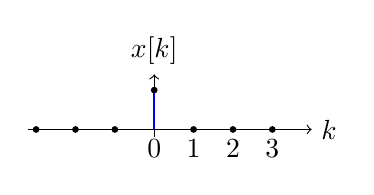
\begin{tikzpicture}[baseline=0.8,scale=0.5]
					      \draw[->] (0,-0.2) -- (0,1.4) node[above]{$x[k]$}; %y
					      \draw[->] (-3.2,0) -- (4,0) node[right]{$k$}; %x
					      \filldraw[black] (-3,0) circle (2pt) {};
					      \filldraw[black] (-2,0) circle (2pt) {};
					      \filldraw[black] (-1,0) circle (2pt) {};
					      \draw[blue, thick] (0,1) -- (0,0) node[below, black]{0}; \filldraw[black] (0,1) circle (2pt) {};
					      \filldraw[black] (1,0) circle (2pt) node[below]{1};
					      \filldraw[black] (2,0) circle (2pt) node[below]{2};
					      \filldraw[black] (3,0) circle (2pt) node[below]{3};
				      \end{tikzpicture}
			      \end{minipage}
		      }
		      Eigenschaften:
		      \begin{itemize}
			      \item neutrales Element der Faltung
			      \item Anregung der Impulsantwort
			      \item besitzt konstantes Spektrum
			      \item Summe ist $\sum^{\infty}_{n=-\infty}\delta(n)=1$
		      \end{itemize}
		      Ausblendeeigenschaft:
		      \[
			      x(n) = \sum_{k=-\infty}^{\infty} x(k)\cdot\delta(n-k)
		      \]
		\item \textbf{Einheitssprung}\\
		      \makebox[\textwidth][c]
		      {
			      \begin{minipage}{0.3\textwidth}
				      \[
					      \varepsilon(n) =
					      \begin{cases}
						      1 & n \geq 0 \\
						      0 & n < 0
					      \end{cases}
				      \]
			      \end{minipage}
			      \begin{minipage}{0.7\textwidth}
				      \centering
				      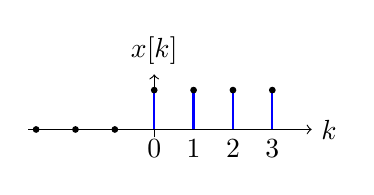
\begin{tikzpicture}[baseline=0.8,scale=0.5]
					      \draw[->] (0,-0.2) -- (0,1.4) node[above]{$x[k]$}; %y
					      \draw[->] (-3.2,0) -- (4,0) node[right]{$k$}; %x
					      \filldraw[black] (-3,0) circle (2pt) {};
					      \filldraw[black] (-2,0) circle (2pt) {};
					      \filldraw[black] (-1,0) circle (2pt) {};
					      \draw[blue, thick] (0,1) -- (0,0) node[below, black]{0}; \filldraw[black] (0,1) circle (2pt) {};
					      \draw[blue, thick] (1,1) -- (1,0) node[below, black]{1}; \filldraw[black] (1,1) circle (2pt) {};
					      \draw[blue, thick] (2,1) -- (2,0) node[below, black]{2}; \filldraw[black] (2,1) circle (2pt) {};
					      \draw[blue, thick] (3,1) -- (3,0) node[below, black]{3}; \filldraw[black] (3,1) circle (2pt) {};
				      \end{tikzpicture}
			      \end{minipage}
		      }
		      Zusammenhang mit Einheitsimpulse:
		      \[
			      \delta(n) = \varepsilon(n) - \varepsilon(n-1)
		      \]
		\item \textbf{Rechteckfolge}\\
		      \makebox[\textwidth][c]
		      {
			      \begin{minipage}{0.3\textwidth}
				      \[
					      \operatorname{rect}(n) =
					      \begin{cases}
						      1 & 0 \leq n < N   \\
						      0 & \texttt{sonst}
					      \end{cases}
				      \]
			      \end{minipage}
			      \begin{minipage}{0.7\textwidth}
				      \centering
				      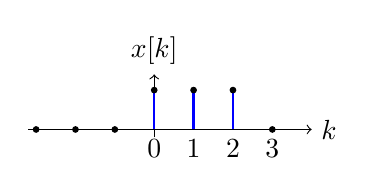
\begin{tikzpicture}[baseline=0.8,scale=0.5]
					      \draw[->] (0,-0.2) -- (0,1.4) node[above]{$x[k]$}; %y
					      \draw[->] (-3.2,0) -- (4,0) node[right]{$k$}; %x
					      \filldraw[black] (-3,0) circle (2pt) {};
					      \filldraw[black] (-2,0) circle (2pt) {};
					      \filldraw[black] (-1,0) circle (2pt) {};
					      \draw[blue, thick] (0,1) -- (0,0) node[below, black]{0}; \filldraw[black] (0,1) circle (2pt) {};
					      \draw[blue, thick] (1,1) -- (1,0) node[below, black]{1}; \filldraw[black] (1,1) circle (2pt) {};
					      \draw[blue, thick] (2,1) -- (2,0) node[below, black]{2}; \filldraw[black] (2,1) circle (2pt) {};
					      \filldraw[black] (3,0) circle (2pt) node[below] {3};
				      \end{tikzpicture}
			      \end{minipage}
		      }
		      Zusammenhang mit Dirac- und Einheitsimpuls:
		      \begin{align*}
			      \operatorname{rect}(n) & = \varepsilon(n) + \varepsilon(n-N)       \\
			                             & = \varepsilon(n) \cdot \varepsilon(N-1-n)
		      \end{align*}
		\item \textbf{Zeitdiskrete Sinus}\\
		      \makebox[\textwidth][c]
		      {
			      \begin{minipage}{0.3\textwidth}
				      \[
					      x(n) = A \cdot \sin(\Omega n+\varphi)
				      \]
			      \end{minipage}
			      \begin{minipage}{0.7\textwidth}
				      \centering
				      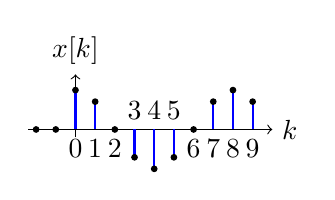
\begin{tikzpicture}[baseline=1,scale=0.5]
					      \draw[->] (0,-0.2) -- (0,1.4) node[above]{$x[k]$}; %y
					      \draw[->] (-1.2,0) -- (5,0) node[right]{$k$}; %x
					      \filldraw[black] (-1,0) circle (2pt) {};
					      \filldraw[black] (-0.5,0) circle (2pt) {};
					      \draw[blue,thick] (0,1) -- (0,0)          node[below, black]{0}; \filldraw[black] (0,1) circle (2pt) {};
					      \draw[blue,thick] (0.5,0.707) -- (0.5,0)  node[below, black]{1}; \filldraw[black] (0.5,0.707) circle (2pt) {};
					      \filldraw[black] (1,0) circle (2pt)              node[below, black]{2};
					      \draw[blue,thick] (1.5,-0.707) -- (1.5,0) node[above, black]{3}; \filldraw[black] (1.5,-0.707) circle (2pt) {};
					      \draw[blue,thick] (2,-1) -- (2,0)         node[above, black]{4}; \filldraw[black] (2,-1) circle (2pt) {};
					      \draw[blue,thick] (2.5,-0.707) -- (2.5,0) node[above, black]{5}; \filldraw[black] (2.5,-0.707) circle (2pt) {};
					      \filldraw[black] (3,0) circle (2pt)              node[below]{6};
					      \draw[blue,thick] (3.5,0.707) -- (3.5,0)  node[below, black]{7}; \filldraw[black] (3.5,0.707) circle (2pt) {};
					      \draw[blue,thick] (4,1) -- (4,0)          node[below, black]{8}; \filldraw[black] (4,1) circle (2pt) {};
					      \draw[blue,thick] (4.5,0.707) -- (4.5,0)  node[below, black]{9}; \filldraw[black] (4.5,0.707) circle (2pt) {};
				      \end{tikzpicture}
			      \end{minipage}
		      }
		      \footnotesize
		      \begin{align*}
			      A       & :\texttt{Amplitude}               \\
			      \Omega  & :\texttt{normierte Kreisfrequenz} \\
			      \varphi & :\texttt{Anfangsphase}
		      \end{align*}
		      \normalsize
		\item \textbf{Exponentialfolge}\\
		      \makebox[\textwidth][c]
		      {
			      \begin{minipage}{0.3\textwidth}
				      \begin{align*}
					      x(n) & = \underline{A} \cdot e^{Sn}                \\
					           & = \underline{A} \cdot e^{(\Sigma+j\Omega)n}
				      \end{align*}
			      \end{minipage}
			      \begin{minipage}{0.7\textwidth}
				      \centering
				      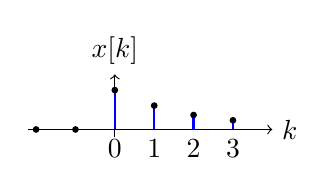
\begin{tikzpicture}[baseline=0.8,scale=0.5]
					      \draw[->] (0,-0.2) -- (0,1.4) node[above]{$x[k]$}; %y
					      \draw[->] (-2.2,0) -- (4,0) node[right]{$k$}; %x
					      \filldraw[black] (-2,0) circle (2pt) {};
					      \filldraw[black] (-1,0) circle (2pt) {};
					      \draw[blue, thick] (0,1) -- (0,0) node[below, black]{0}; \filldraw[black] (0,1) circle (2pt) {};
					      \draw[blue, thick] (1,0.606) -- (1,0) node[below, black]{1}; \filldraw[black] (1,0.606) circle (2pt) {};
					      \draw[blue, thick] (2,0.367) -- (2,0) node[below, black]{2}; \filldraw[black] (2,0.367) circle (2pt) {};
					      \draw[blue, thick] (3,0.233) -- (3,0) node[below, black]{3}; \filldraw[black] (3,0.233) circle (2pt) {};
				      \end{tikzpicture}
			      \end{minipage}
		      }
		      \begin{align*}
			      S                                       & = \Sigma+j\Omega        \\
			      \texttt{Amplitudenänderung }\Sigma      & = \sigma T = \sigma/f_A \\
			      \texttt{normierte Kreisfrequenz }\Omega & = \omega T =  2\pi f_A
		      \end{align*}
	\end{itemize}
\end{mdframed}
\subsection{Abtasttheorem im Fequenzbereich}
Nur wenn das Eingangssignal auf $\omega_g$ bandbegrenzt und die Abtastfrequenz $\omega_a  \geq
	2\omega_g$ ist, kommt es nicht zu spektralen Überlappungen (= Aliasing).

Aliasing führt zu zusätzlichen Abtastwerten nicht mehr rekonstruieren lässt.

\centering
\includegraphics[width=0.5\columnwidth]{Bilder/Abtasttheorem_Uebrlappung}

\raggedright
\subsection{Elementare Zeitdiskrete Systeme}
\subsubsection{Definition}
Ein System, das sowohl linear, als auch zeitinvariant ist, nennen wir ein
lineares zeitinvariantes System, oder kurz LTI-System

\subsubsection{Kausalität und Stabilität}
\begin{itemize}
	\item \textbf{Kausal}:
	      wenn die Anzahl der Pole (= Grad des Nennerpolynoms) größer gleich
	      der Anzahl der Nullstellen (= Grad des Zählerpolynoms) ist.
	\item \textbf{Stabil}:
	      wenn der Einheitskreis zum Konvergenzbereich gehört
\end{itemize}

\begin{center}
	\fbox{\parbox{.9\columnwidth}{Liegen alle Pole innerhalb des Einheitskreises,
			so ist das LTI-System kausal und stabil!}}
\end{center}

\subsubsection{Klassifizierung von Systemen}
% Die mathematischen Beschreibung fehlen. wurden nie gebraucht während lernen. Kap6S63 6.5.7
\begin{mdframed}[style=exercise]
	\begin{itemize}
		\item \textbf{Transversale Systeme:}\\
		      Der Ausgang wird nicht auf den Eingang zurückgeführt\\
		      $\Rightarrow$ $a_k=0 \texttt{ für } k>0$\\
		      $\Rightarrow$ alle Pole liegen im Ursprung

		      \makebox[\columnwidth][c]{
			      \begin{minipage}{0.4\textwidth}
				      \includegraphics[width=0.7\textwidth]{Bilder/Transversale_Systeme_}
			      \end{minipage}
			      \hspace{-1em}
			      \begin{minipage}{0.6\textwidth}
				      \includegraphics[width=0.8\textwidth]{Bilder/Transversale_Systeme_SG}
			      \end{minipage}
		      }
		\item \textbf{Rekursive Systeme:}\\
		      Der aktuelle Ausgangswert hängt nur vom aktuellen Eingangswert
		      und früheren Ausgangswerten ab.\\
		      $\Rightarrow$ $b_k=0 \texttt{ für } k>0$\\
		      $\Rightarrow$ alle Nullstellen liegen im Ursprung

		      \makebox[\columnwidth][c]{
			      \begin{minipage}{0.4\textwidth}
				      \includegraphics[width=0.7\textwidth]{Bilder/Rekursive_Systeme}
			      \end{minipage}
			      \hspace{-1em}
			      \begin{minipage}{0.6\textwidth}
				      \includegraphics[width=0.8\textwidth]{Bilder/Rekursive_Systeme_SG}
			      \end{minipage}
		      }
	\end{itemize}
\end{mdframed}

Systeme nach der Länge der Impulsantwort
\begin{itemize}
	\item \textbf{Finite Impulse Response (FIR) Systeme:}\\
	      \bulletpt haben \underline{endlich} lange Impulsantworten\\
	      \bulletpt synonym zum Begriff transversales System\\
	      \bulletpt endlich lange Impulsantworten lassen sich auch mit
	      transversal-rekursiven Systemen erreichen
	\item \textbf{Infinite Impulse Response (IIR) Systeme:}\\
	      \bulletpt haben \underline{unendlich} lange Impulsantworten\\
	      \bulletpt synonym zum Begriff rekursives System
\end{itemize}
